\documentclass{beamer}
\usetheme{default}
\usepackage{amsmath, amsfonts, amsthm} % basic math packages
\usepackage{tikz} % for making illustrations
\usetikzlibrary{shapes.arrows, arrows, decorations.markings, positioning}
\usetikzlibrary{calc}
\usetikzlibrary{3d}
\usepackage{graphicx} % for importing images
\usepackage{xcolor} % more color options
\usepackage{colortbl}
\usepackage{multicol} % for making two-column lists
\usepackage{hyperref} % for hyperlinking
%\hypersetup{colorlinks=true, urlcolor=cyan,}
\usepackage{mathabx}
\usepackage{cleveref}
\usepackage{subfig}
\usepackage{array}
\usepackage{wrapfig}
\usepackage{bbm}
\usepackage{fancyhdr}
\usepackage{algorithm, algorithmicx, algpseudocode}
\usepackage{stmaryrd}
\usepackage{physics}
\AtBeginSection[]
{
	\begin{frame}
		\frametitle{Table of Contents}
		\tableofcontents[currentsection]
	\end{frame}
}

\title{A \LaTeX'ed solution to B-tree insertion and deletion.}
\author{Mitchell Scott (mtscot4)}
\begin{document}
\begin{frame}[plain]
    \maketitle
\end{frame}
\begin{frame}{B-Tree Insertion and Deletion Assignments}
	\tableofcontents
\end{frame}
\section{Assignment 3-1: Insert}
\begin{frame}{For $m=2$, and the below B-tree, insert the keys 25, 17, 42 and 29, in this order.}
		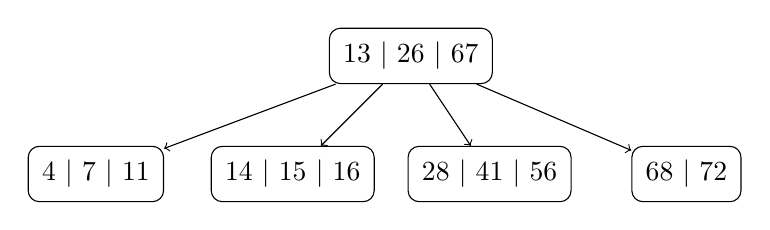
\begin{tikzpicture}
			\draw (0,0)     node[inner sep=5pt,draw, rounded corners] (c1){$4 \ | \  7\  |\  11$}
			(2.5cm,0em) node[inner sep=5pt,draw,rounded corners] (c2) {$14 \ | \ 15\ |\ 16$}
			(5cm,0em) node[inner sep=5pt,draw, rounded corners] (c3) {$28\ |\ 41\ |\ 56$}%node[fill=yellow!80!black]   {default};
			(7.5cm,0em) node[inner sep=5pt,draw,rounded corners] (c4){$68\ |\ 72$}
			(4cm,1.5cm) node[inner sep=5pt,draw,rounded corners](r1) {$13 \ | \ 26\ |\ 67$};
			
			\draw[->] (r1) -- (c1);
			\draw[->] (r1) -- (c2);
			\draw[->] (r1) -- (c3);
			\draw[->] (r1) -- (c4);
		\end{tikzpicture}
	\end{frame}
	\begin{frame}{25 is inserted into currentNode, currentNode is checked for overflow. Since $4\leq 2m=4$, there is no overflow.}
		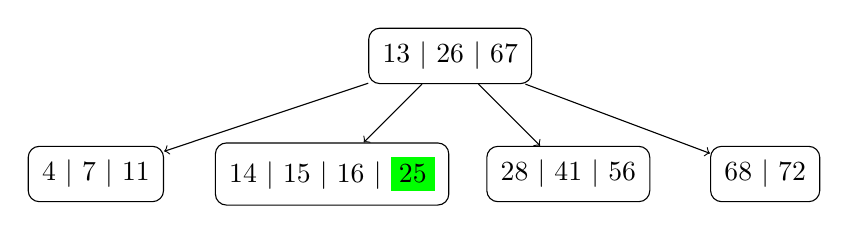
\begin{tikzpicture}
			\draw (-.5,-3.5cm)     node[inner sep=5pt,draw, rounded corners] (c1){$4 \ | \  7\  |\  11$}
			(2.5cm,-3.5cm) node[inner sep=5pt,draw,rounded corners] (c2) {$14 \ | \ 15\ |\ 16\ | \ \colorbox{green}{25}$}
			(5.5cm,-3.5cm) node[inner sep=5pt,draw, rounded corners] (c3) {$28\ |\ 41\ |\ 56$}%
			(8cm,-3.5cm) node[inner sep=5pt,draw,rounded corners] (c4){$68\ |\ 72$}
			(4cm,-2cm) node[inner sep=5pt,draw,rounded corners](r1) {$13 \ | \ 26\ |\ 67$};
			
			\draw[->] (r1) -- (c1);
			\draw[->] (r1) -- (c2);
			\draw[->] (r1) -- (c3);
			\draw[->] (r1) -- (c4);
		\end{tikzpicture}
	
\end{frame}
\begin{frame}{17 is inserted into currentNode, currentNode is checked for overflow. $5>2m=4$, so overflow, as it violates the B-tree property.}
		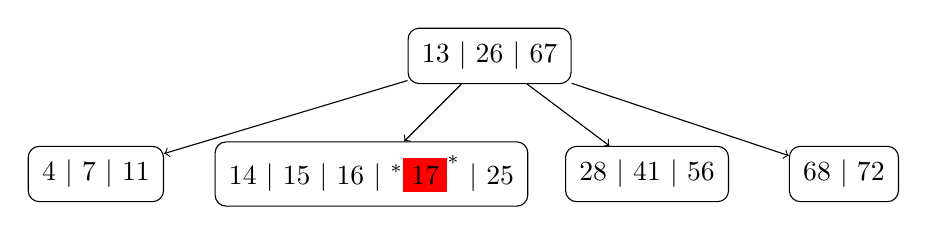
\begin{tikzpicture}
		\draw (-1.0,-3.5cm)     node[inner sep=5pt,draw, rounded corners] (c1){$4 \ | \  7\  |\  11$}
		(2.5cm,-3.5cm) node[inner sep=5pt,draw,rounded corners] (c2) {$14 \ | \ 15\ |\ 16\ |\ ^\ast \colorbox{red}{17}^\ast\ |\ 25$}
		(6.0cm,-3.5cm) node[inner sep=5pt,draw, rounded corners] (c3) {$28\ |\ 41\ |\ 56$}%
		(8.5cm,-3.5cm) node[inner sep=5pt,draw,rounded corners] (c4){$68\ |\ 72$}
		(4cm,-2cm) node[inner sep=5pt,draw,rounded corners](r1) {$13 \ | \ 26\ |\ 67$};
		
		\draw[->] (r1) -- (c1);
		\draw[->] (r1) -- (c2);
		\draw[->] (r1) -- (c3);
		\draw[->] (r1) -- (c4);
	\end{tikzpicture}
\end{frame}

\begin{frame}{16 is found to be the median of the keys of currentNode, so we move 13 from currentNode to \texttt{Parent}.}
	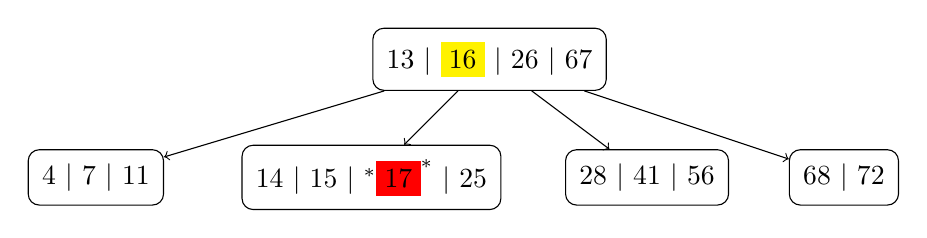
\begin{tikzpicture}
		\draw (-1.0,-3.5cm)     node[inner sep=5pt,draw, rounded corners] (c1){$4 \ | \  7\  |\  11$}
		(2.5cm,-3.5cm) node[inner sep=5pt,draw,rounded corners] (c2) {$14 \ | \ 15\  | \ ^\ast\colorbox{red}{17}^\ast\ |\ 25$}
		(6.0cm,-3.5cm) node[inner sep=5pt,draw, rounded corners] (c3) {$28\ |\ 41\ |\ 56$}%
		(8.5cm,-3.5cm) node[inner sep=5pt,draw,rounded corners] (c4){$68\ |\ 72$}
		(4cm,-2cm) node[inner sep=5pt,draw,rounded corners](r1) {$13 \ | \ \colorbox{yellow}{16} \ | \ 26\ |\ 67$};
		
		\draw[->] (r1) -- (c1);
		\draw[->] (r1) -- (c2);
		\draw[->] (r1) -- (c3);
		\draw[->] (r1) -- (c4);
	\end{tikzpicture}
\end{frame}


\begin{frame}{Now, \texttt{parent} has the wrong number of pointers, as four keys should have five pointers. We split  \texttt{`currrentNode'} into \texttt{`leftNode'} and \texttt{`rightNode'} .}
	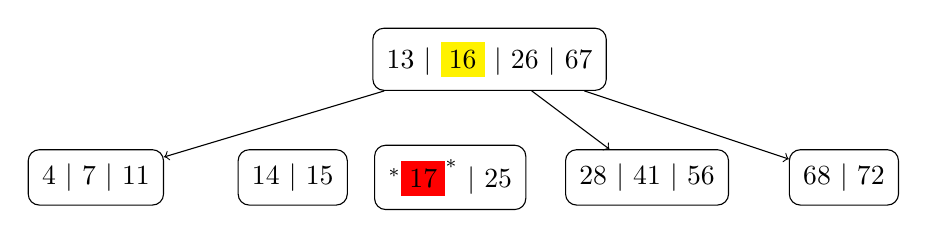
\begin{tikzpicture}
		\draw (-1.0,-3.5cm)     node[inner sep=5pt,draw, rounded corners] (c1){$4 \ | \  7\  |\  11$}
		(1.5cm,-3.5cm) node[inner sep=5pt,draw,rounded corners] (c2) {$14 \ | \ 15$}
		(3.5cm,-3.5cm) node[inner sep = 5pt, draw, rounded corners] (c3) {  $^\ast\colorbox{red}{17}^\ast\ |\ 25$}
		(6.0cm,-3.5cm) node[inner sep=5pt,draw, rounded corners] (c4) {$28\ |\ 41\ |\ 56$}%
		(8.5cm,-3.5cm) node[inner sep=5pt,draw,rounded corners] (c5){$68\ |\ 72$}
		(4cm,-2cm) node[inner sep=5pt,draw,rounded corners](r1) {$13 \ | \ \colorbox{yellow}{16} \ | \ 26\ |\ 67$};
		
		\draw[->] (r1) -- (c1);
		\draw[->] (r1) -- (c4);
		\draw[->] (r1) -- (c5);
	\end{tikzpicture}
\end{frame}

\begin{frame}{We add the left and right pointer to \texttt{leftNode} and \texttt{rightNode}, respectively. Lastly, since the root has grown, we check for overflow. Since $4\leq 2m=4$ keys, there is no overflow. We have finally inserted 17.}
	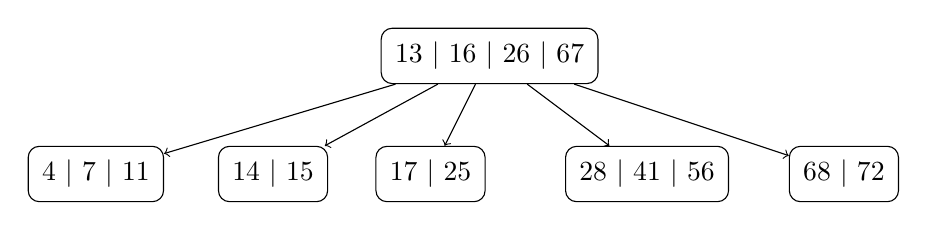
\begin{tikzpicture}
		\draw (-1.0,-3.5cm)     node[inner sep=5pt,draw, rounded corners] (c1){$4 \ | \  7\  |\  11$}
		(1.25cm,-3.5cm) node[inner sep=5pt,draw,rounded corners] (c2) {$14 \ | \ 15$}
		(3.25cm,-3.5cm) node[inner sep = 5pt, draw, rounded corners] (c3) {  $17\  |\ 25$}
		(6.0cm,-3.5cm) node[inner sep=5pt,draw, rounded corners] (c4) {$28\ |\ 41\ |\ 56$}%
		(8.5cm,-3.5cm) node[inner sep=5pt,draw,rounded corners] (c5){$68\ |\ 72$}
		(4cm,-2cm) node[inner sep=5pt,draw,rounded corners](r1) {$13 \ | \ 16 \ | \ 26\ |\ 67$};
		
		\draw[->] (r1) -- (c1);
		\draw[->] (r1) -- (c2);
		\draw[->] (r1) -- (c3);
		\draw[->] (r1) -- (c4);
		\draw[->] (r1) -- (c5);
	\end{tikzpicture}
\end{frame}

\begin{frame}{Now we seek to insert 42. Since the new \texttt{currentNode} has $4\leq2m=4$ keys, we don't have overflow, so we are done.}
	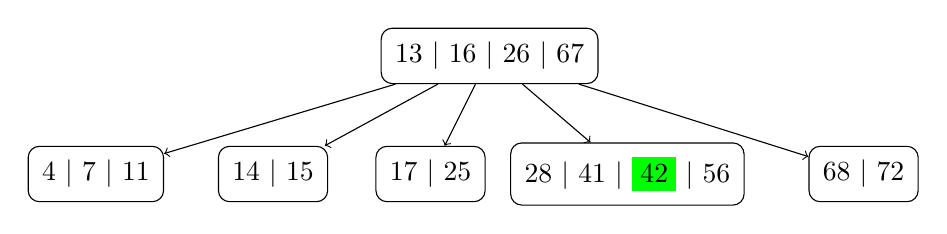
\begin{tikzpicture}
		\draw (-1.0,-3.5cm)     node[inner sep=5pt,draw, rounded corners] (c1){$4 \ | \  7\  |\  11$}
		(1.25cm,-3.5cm) node[inner sep=5pt,draw,rounded corners] (c2) {$14 \ | \ 15$}
		(3.25cm,-3.5cm) node[inner sep = 5pt, draw, rounded corners] (c3) {  $17\  |\ 25$}
		(5.75cm,-3.5cm) node[inner sep=5pt,draw, rounded corners] (c4) {$28\ |\ 41\ | \ \colorbox{green}{42}\ | \ 56$}%
		(8.75cm,-3.5cm) node[inner sep=5pt,draw,rounded corners] (c5){$68\ |\ 72$}
		(4cm,-2cm) node[inner sep=5pt,draw,rounded corners](r1) {$13 \ | \ 16 \ | \ 26\ |\ 67$};
		
		\draw[->] (r1) -- (c1);
		\draw[->] (r1) -- (c2);
		\draw[->] (r1) -- (c3);
		\draw[->] (r1) -- (c4);
		\draw[->] (r1) -- (c5);
	\end{tikzpicture}
\end{frame}

\begin{frame}{Lastly, we seek to add 29. We insert into \texttt{currentNode}, but observe that \texttt{currentNode} is overflowing as it has $5> 2m = 4$ keys. }
	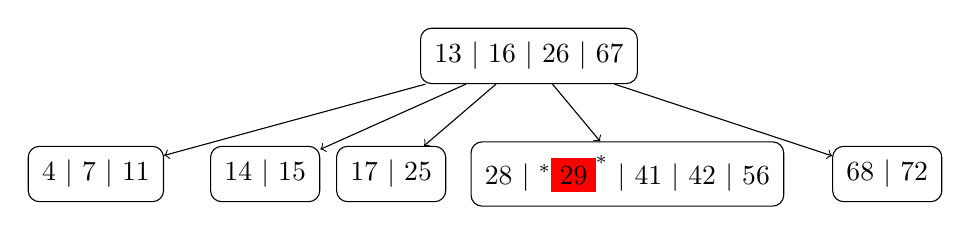
\begin{tikzpicture}
		\draw (-1.5,-3.5cm)     node[inner sep=5pt,draw, rounded corners] (c1){$4 \ | \  7\  |\  11$}
		(0.65cm,-3.5cm) node[inner sep=5pt,draw,rounded corners] (c2) {$14 \ | \ 15$}
		(2.25cm,-3.5cm) node[inner sep = 5pt, draw, rounded corners] (c3) {  $17\  |\ 25$}
		(5.25cm,-3.5cm) node[inner sep=5pt,draw, rounded corners] (c4) {$28\ |\ ^\ast\colorbox{red}{29}^\ast\ | \ 41\ | \ 42\ | \ 56$}%
		(8.55cm,-3.5cm) node[inner sep=5pt,draw,rounded corners] (c5){$68\ |\ 72$}
		(4cm,-2cm) node[inner sep=5pt,draw,rounded corners](r1) {$13 \ | \ 16 \ | \ 26\ |\ 67$};
		
		\draw[->] (r1) -- (c1);
		\draw[->] (r1) -- (c2);
		\draw[->] (r1) -- (c3);
		\draw[->] (r1) -- (c4);
		\draw[->] (r1) -- (c5);
	\end{tikzpicture}
\end{frame}
\begin{frame}{41 is the median of \texttt{currentNode} so we move it to \texttt{parent}. The rest of the node is split as we need another pointer coming from \texttt{parent}. }
	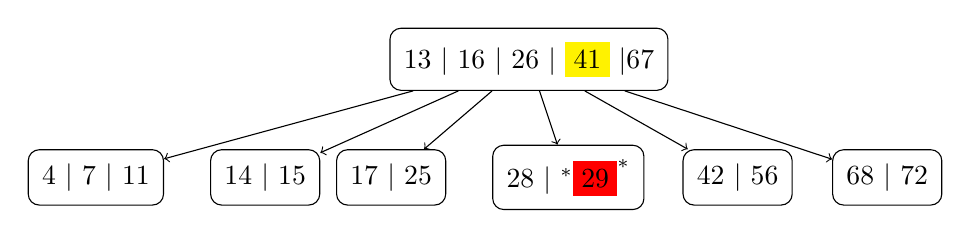
\begin{tikzpicture}
		\draw (-1.5,-3.5cm)     node[inner sep=5pt,draw, rounded corners] (c1){$4 \ | \  7\  |\  11$}
		(0.65cm,-3.5cm) node[inner sep=5pt,draw,rounded corners] (c2) {$14 \ | \ 15$}
		(2.25cm,-3.5cm) node[inner sep = 5pt, draw, rounded corners] (c3) {  $17\  |\ 25$}
		(4.5cm,-3.5cm) node[inner sep=5pt,draw, rounded corners] (c4) {$28\ |\ ^\ast\colorbox{red}{29}^\ast$}
		(6.65cm, -3.5cm) node[inner sep=5pt, draw, rounded corners] (c5){$42\ | \ 56$}%
		(8.55cm,-3.5cm) node[inner sep=5pt,draw,rounded corners] (c6){$68\ |\ 72$}
		(4cm,-2cm) node[inner sep=5pt,draw,rounded corners](r1) {$13 \ | \ 16 \ | \ 26\ |\ \colorbox{yellow}{41}\ | 67$};
		
		\draw[->] (r1) -- (c1);
		\draw[->] (r1) -- (c2);
		\draw[->] (r1) -- (c3);
		\draw[->] (r1) -- (c4);
		\draw[->] (r1) -- (c5);
		\draw[->] (r1) -- (c6);
	\end{tikzpicture}
\end{frame}
\begin{frame}{Lastly, we have overflow at the root, so we follow the same precedure, where we find the median, and move to \texttt{parent}, or becoming the new root in this case. }
	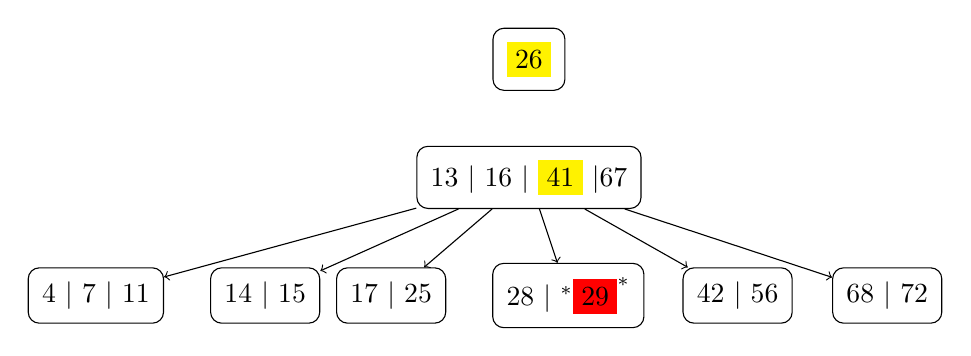
\begin{tikzpicture}
		\draw (-1.5,-3.5cm)     node[inner sep=5pt,draw, rounded corners] (c1){$4 \ | \  7\  |\  11$}
		(0.65cm,-3.5cm) node[inner sep=5pt,draw,rounded corners] (c2) {$14 \ | \ 15$}
		(2.25cm,-3.5cm) node[inner sep = 5pt, draw, rounded corners] (c3) {  $17\  |\ 25$}
		(4.5cm,-3.5cm) node[inner sep=5pt,draw, rounded corners] (c4) {$28\ |\ ^\ast\colorbox{red}{29}^\ast$}
		(6.65cm, -3.5cm) node[inner sep=5pt, draw, rounded corners] (c5){$42\ | \ 56$}%
		(8.55cm,-3.5cm) node[inner sep=5pt,draw,rounded corners] (c6){$68\ |\ 72$}
		(4cm,-2cm) node[inner sep=5pt,draw,rounded corners](r1) {$13 \ | \ 16 \ |\ \colorbox{yellow}{41}\ | 67$}
		(4cm, -0.5cm) node[inner sep = 5pt, draw, rounded corners] (r0) {$\colorbox{yellow}{26}$};
		
		\draw[->] (r1) -- (c1);
		\draw[->] (r1) -- (c2);
		\draw[->] (r1) -- (c3);
		\draw[->] (r1) -- (c4);
		\draw[->] (r1) -- (c5);
		\draw[->] (r1) -- (c6);
	\end{tikzpicture}
\end{frame}
\begin{frame}{We split the remaining node, and they are now children of \texttt{newRoot}. A keen observer, such as \textsc{Random Cat}, might suspect underflow at the new root, but the root doesn't have a minimum number of keys, so we are done! }
	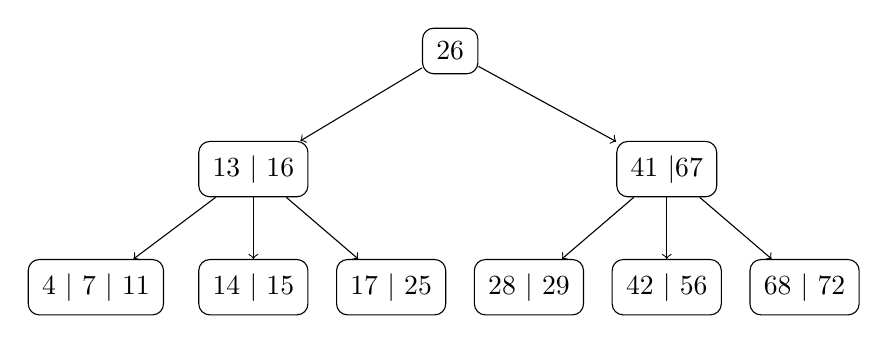
\begin{tikzpicture}
		\draw (-1.5,-3.5cm)     node[inner sep=5pt,draw, rounded corners] (c1){$4 \ | \  7\  |\  11$}
		(0.5cm,-3.5cm) node[inner sep=5pt,draw,rounded corners] (c2) {$14 \ | \ 15$}
		(2.25cm,-3.5cm) node[inner sep = 5pt, draw, rounded corners] (c3) {  $17\  |\ 25$}
		(4cm,-3.5cm) node[inner sep=5pt,draw, rounded corners] (c4) {$28\ |\ 29$}
		(5.75cm, -3.5cm) node[inner sep=5pt, draw, rounded corners] (c5){$42\ | \ 56$}%
		(7.5cm,-3.5cm) node[inner sep=5pt,draw,rounded corners] (c6){$68\ |\ 72$}
		(0.5cm,-2cm) node[inner sep=5pt,draw,rounded corners](r1) {$13 \ | \ 16$}
		 (5.75cm, -2cm) node[inner sep = 5pt,draw,rounded corners](r2) {$ 41\ | 67$}
		(3.0cm, -0.5cm) node[inner sep = 5pt, draw, rounded corners] (r0) {$26$};
		
		\draw[->] (r1) -- (c1);
		\draw[->] (r1) -- (c2);
		\draw[->] (r1) -- (c3);
		\draw[->] (r2) -- (c4);
		\draw[->] (r2) -- (c5);
		\draw[->] (r2) -- (c6);
		\draw[->] (r0) -- (r1);
		\draw[->] (r0) -- (r2);
	\end{tikzpicture}
\end{frame}
\section{Assignment 3-1: Deletion}
\begin{frame}{For $m=2$, and the below B-tree, delete the keys 18,14,21, and 1, in this order.}
	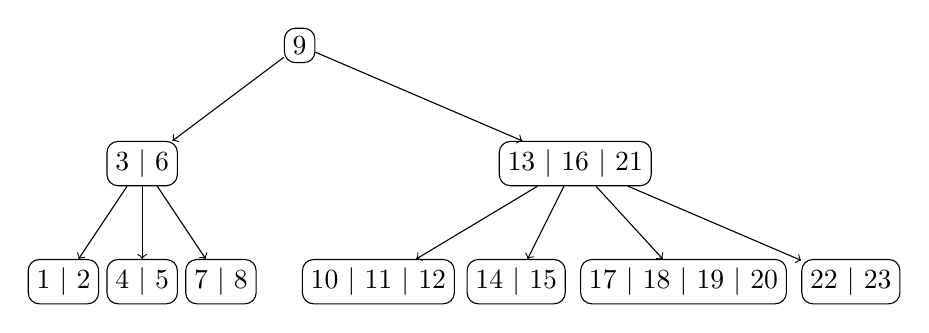
\begin{tikzpicture}
		\draw (1cm,2.0cm) node[inner sep = 3pt,draw,rounded corners] (r1){$9$}
		(-1.0cm, 0.5cm) node[inner sep = 3pt, draw,rounded corners] (lc1) {$3\ | \ 6$}
		(-2cm, -1.0cm) node[inner sep = 3pt, draw,rounded corners] (llc1) {$1\ | \ 2$}
		(-1cm, -1.0cm) node[inner sep = 3pt, draw,rounded corners] (llc2) {$4\ | \ 5$}
		(0cm, -1.0cm) node[inner sep = 3pt, draw,rounded corners] (llc3) {$7\ | \ 8$}
		(4.5cm, 0.5cm) node[inner sep = 3pt, draw,rounded corners] (rc1) {$13\ | \ 16 \ | \ 21$}
		(2cm, -1.0cm) node[inner sep = 3pt, draw,rounded corners] (rrc1) {$10\ | \ 11\ | \ 12$}
		(3.75cm, -1.0cm) node[inner sep = 3pt, draw,rounded corners] (rrc2) {$14\ | \ 15$}
		(5.875cm, -1.0cm) node[inner sep = 3pt, draw,rounded corners] (rrc3) {$17\ | \ 18\ | \ 19\ | \ 20$}
		(8cm, -1.0cm) node[inner sep = 3pt, draw,rounded corners] (rrc4) {$22\ | \ 23$};
		
		\draw[->] (r1) -- (lc1);
		\draw[->] (r1) -- (rc1);
		\draw[->] (lc1) -- (llc1);
		\draw[->] (lc1) -- (llc2);
		\draw[->] (lc1) -- (llc3);
		\draw[->] (rc1) -- (rrc1);
		\draw[->] (rc1) -- (rrc2);
		\draw[->] (rc1) -- (rrc3);
		\draw[->] (rc1) -- (rrc4);
	\end{tikzpicture}
\end{frame}
\begin{frame}{Since 18 is a leaf node, it is deleted at \texttt{currentNode}. Then we check \texttt{currentNode} for underflow. Since $3>m=2$, there is no underflow, so no additional work to delete 18.}
	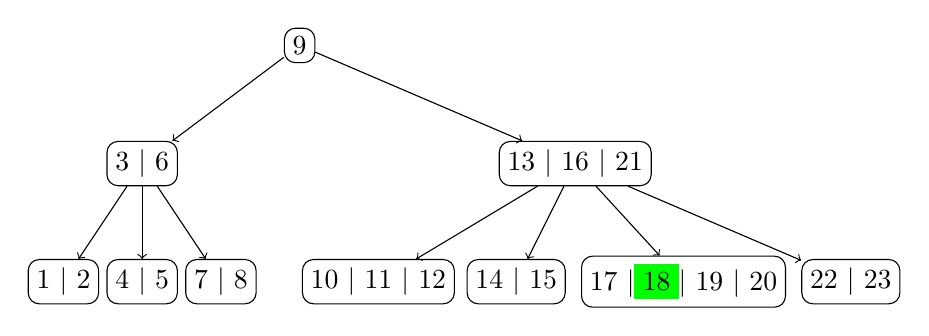
\begin{tikzpicture}
		\draw (1cm,2.0cm) node[inner sep = 3pt,draw,rounded corners] (r1){$9$}
		(-1.0cm, 0.5cm) node[inner sep = 3pt, draw,rounded corners] (lc1) {$3\ | \ 6$}
		(-2cm, -1.0cm) node[inner sep = 3pt, draw,rounded corners] (llc1) {$1\ | \ 2$}
		(-1cm, -1.0cm) node[inner sep = 3pt, draw,rounded corners] (llc2) {$4\ | \ 5$}
		(0cm, -1.0cm) node[inner sep = 3pt, draw,rounded corners] (llc3) {$7\ | \ 8$}
		(4.5cm, 0.5cm) node[inner sep = 3pt, draw,rounded corners] (rc1) {$13\ | \ 16 \ | \ 21$}
		(2cm, -1.0cm) node[inner sep = 3pt, draw,rounded corners] (rrc1) {$10\ | \ 11\ | \ 12$}
		(3.75cm, -1.0cm) node[inner sep = 3pt, draw,rounded corners] (rrc2) {$14\ | \ 15$}
		(5.875cm, -1.0cm) node[inner sep = 3pt, draw,rounded corners] (rrc3) {$17\ | \colorbox{green}{18}| \ 19\ | \ 20$}
		(8cm, -1.0cm) node[inner sep = 3pt, draw,rounded corners] (rrc4) {$22\ | \ 23$};
		
		\draw[->] (r1) -- (lc1);
		\draw[->] (r1) -- (rc1);
		\draw[->] (lc1) -- (llc1);
		\draw[->] (lc1) -- (llc2);
		\draw[->] (lc1) -- (llc3);
		\draw[->] (rc1) -- (rrc1);
		\draw[->] (rc1) -- (rrc2);
		\draw[->] (rc1) -- (rrc3);
		\draw[->] (rc1) -- (rrc4);
	\end{tikzpicture}
\end{frame}
\begin{frame}{14 is deleted at \texttt{currentNode}, so we check \texttt{currentNode} for underflow.}
	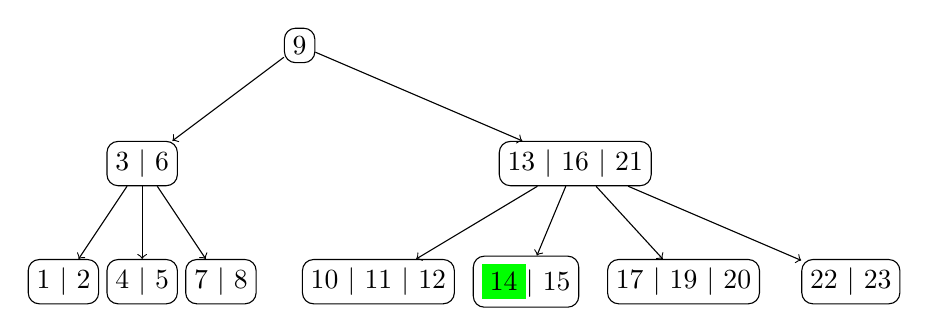
\begin{tikzpicture}
		\draw (1cm,2.0cm) node[inner sep = 3pt,draw,rounded corners] (r1){$9$}
		(-1.0cm, 0.5cm) node[inner sep = 3pt, draw,rounded corners] (lc1) {$3\ | \ 6$}
		(-2cm, -1.0cm) node[inner sep = 3pt, draw,rounded corners] (llc1) {$1\ | \ 2$}
		(-1cm, -1.0cm) node[inner sep = 3pt, draw,rounded corners] (llc2) {$4\ | \ 5$}
		(0cm, -1.0cm) node[inner sep = 3pt, draw,rounded corners] (llc3) {$7\ | \ 8$}
		(4.5cm, 0.5cm) node[inner sep = 3pt, draw,rounded corners] (rc1) {$13\ | \ 16 \ | \ 21$}
		(2cm, -1.0cm) node[inner sep = 3pt, draw,rounded corners] (rrc1) {$10\ | \ 11\ | \ 12$}
		(3.875cm, -1.0cm) node[inner sep = 3pt, draw,rounded corners] (rrc2) {$\colorbox{green}{14}| \ 15$}
		(5.875cm, -1.0cm) node[inner sep = 3pt, draw,rounded corners] (rrc3) {$17\ | \ 19\ | \ 20$}
		(8cm, -1.0cm) node[inner sep = 3pt, draw,rounded corners] (rrc4) {$22\ | \ 23$};
		
		\draw[->] (r1) -- (lc1);
		\draw[->] (r1) -- (rc1);
		\draw[->] (lc1) -- (llc1);
		\draw[->] (lc1) -- (llc2);
		\draw[->] (lc1) -- (llc3);
		\draw[->] (rc1) -- (rrc1);
		\draw[->] (rc1) -- (rrc2);
		\draw[->] (rc1) -- (rrc3);
		\draw[->] (rc1) -- (rrc4);
	\end{tikzpicture}
\end{frame}
\begin{frame}{\texttt{currentNode} is a leaf node that is underflowing as $1<m=2$ key. We observe that \texttt{rightSibling} has $3\geq m=2$ nodes, so we borrow from it. }
	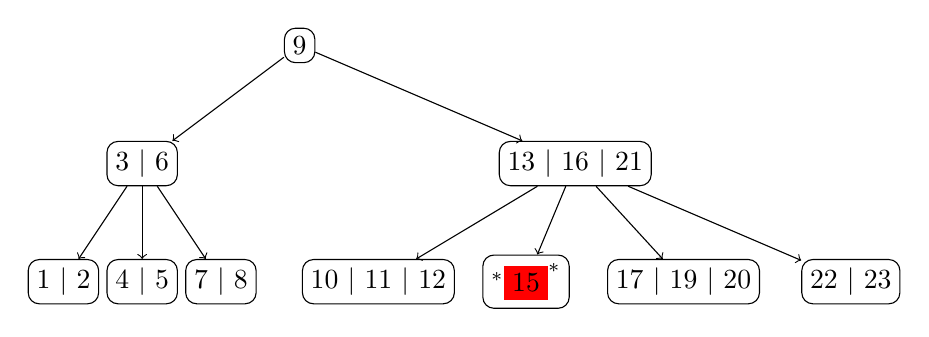
\begin{tikzpicture}
		\draw (1cm,2.0cm) node[inner sep = 3pt,draw,rounded corners] (r1){$9$}
		(-1.0cm, 0.5cm) node[inner sep = 3pt, draw,rounded corners] (lc1) {$3\ | \ 6$}
		(-2cm, -1.0cm) node[inner sep = 3pt, draw,rounded corners] (llc1) {$1\ | \ 2$}
		(-1cm, -1.0cm) node[inner sep = 3pt, draw,rounded corners] (llc2) {$4\ | \ 5$}
		(0cm, -1.0cm) node[inner sep = 3pt, draw,rounded corners] (llc3) {$7\ | \ 8$}
		(4.5cm, 0.5cm) node[inner sep = 3pt, draw,rounded corners] (rc1) {$13\ | \ 16 \ | \ 21$}
		(2cm, -1.0cm) node[inner sep = 3pt, draw,rounded corners] (rrc1) {$10\ | \ 11\ | \ 12$}
		(3.875cm, -1.0cm) node[inner sep = 3pt, draw,rounded corners] (rrc2) {$^\ast\colorbox{red}{15}^\ast$}
		(5.875cm, -1.0cm) node[inner sep = 3pt, draw,rounded corners] (rrc3) {$17\ | \ 19\ | \ 20$}
		(8cm, -1.0cm) node[inner sep = 3pt, draw,rounded corners] (rrc4) {$22\ | \ 23$};
		
		\draw[->] (r1) -- (lc1);
		\draw[->] (r1) -- (rc1);
		\draw[->] (lc1) -- (llc1);
		\draw[->] (lc1) -- (llc2);
		\draw[->] (lc1) -- (llc3);
		\draw[->] (rc1) -- (rrc1);
		\draw[->] (rc1) -- (rrc2);
		\draw[->] (rc1) -- (rrc3);
		\draw[->] (rc1) -- (rrc4);
	\end{tikzpicture}
\end{frame}
\begin{frame}{We perform a rotation to borrow from \texttt{rightSibling}. 17 goes from \texttt{rightSibling} to \texttt{parent}, which allows 16 to go from \texttt{parent} to \texttt{currentNode}. Done.}
	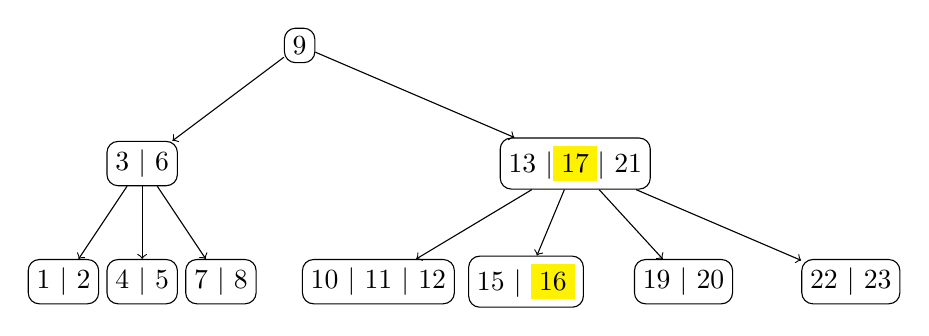
\begin{tikzpicture}
		\draw (1cm,2.0cm) node[inner sep = 3pt,draw,rounded corners] (r1){$9$}
		(-1.0cm, 0.5cm) node[inner sep = 3pt, draw,rounded corners] (lc1) {$3\ | \ 6$}
		(-2cm, -1.0cm) node[inner sep = 3pt, draw,rounded corners] (llc1) {$1\ | \ 2$}
		(-1cm, -1.0cm) node[inner sep = 3pt, draw,rounded corners] (llc2) {$4\ | \ 5$}
		(0cm, -1.0cm) node[inner sep = 3pt, draw,rounded corners] (llc3) {$7\ | \ 8$}
		(4.5cm, 0.5cm) node[inner sep = 3pt, draw,rounded corners] (rc1) {$13\ | \colorbox{yellow}{17} | \ 21$}
		(2cm, -1.0cm) node[inner sep = 3pt, draw,rounded corners] (rrc1) {$10\ | \ 11\ | \ 12$}
		(3.875cm, -1.0cm) node[inner sep = 3pt, draw,rounded corners] (rrc2) {$15\ | \ \colorbox{yellow}{16}$}
		(5.875cm, -1.0cm) node[inner sep = 3pt, draw,rounded corners] (rrc3) {$ 19\ | \ 20$}
		(8cm, -1.0cm) node[inner sep = 3pt, draw,rounded corners] (rrc4) {$22\ | \ 23$};
		
		\draw[->] (r1) -- (lc1);
		\draw[->] (r1) -- (rc1);
		\draw[->] (lc1) -- (llc1);
		\draw[->] (lc1) -- (llc2);
		\draw[->] (lc1) -- (llc3);
		\draw[->] (rc1) -- (rrc1);
		\draw[->] (rc1) -- (rrc2);
		\draw[->] (rc1) -- (rrc3);
		\draw[->] (rc1) -- (rrc4);
	\end{tikzpicture}
\end{frame}
\begin{frame}{To delete 21, which is a branch node, we must switch it with the next largest key, 22, which is guarenteed to be a leaf node.}
	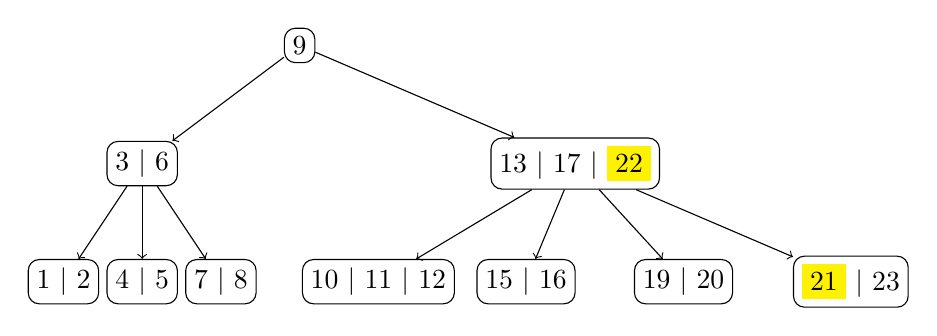
\begin{tikzpicture}
		\draw (1cm,2.0cm) node[inner sep = 3pt,draw,rounded corners] (r1){$9$}
		(-1.0cm, 0.5cm) node[inner sep = 3pt, draw,rounded corners] (lc1) {$3\ | \ 6$}
		(-2cm, -1.0cm) node[inner sep = 3pt, draw,rounded corners] (llc1) {$1\ | \ 2$}
		(-1cm, -1.0cm) node[inner sep = 3pt, draw,rounded corners] (llc2) {$4\ | \ 5$}
		(0cm, -1.0cm) node[inner sep = 3pt, draw,rounded corners] (llc3) {$7\ | \ 8$}
		(4.5cm, 0.5cm) node[inner sep = 3pt, draw,rounded corners] (rc1) {$13\ |\ 17 \ | \ \colorbox{yellow}{22}$}
		(2cm, -1.0cm) node[inner sep = 3pt, draw,rounded corners] (rrc1) {$10\ | \ 11\ | \ 12$}
		(3.875cm, -1.0cm) node[inner sep = 3pt, draw,rounded corners] (rrc2) {$15\ | \ 16$}
		(5.875cm, -1.0cm) node[inner sep = 3pt, draw,rounded corners] (rrc3) {$ 19\ | \ 20$}
		(8cm, -1.0cm) node[inner sep = 3pt, draw,rounded corners] (rrc4) {$\colorbox{yellow}{21}\ | \ 23$};
		
		\draw[->] (r1) -- (lc1);
		\draw[->] (r1) -- (rc1);
		\draw[->] (lc1) -- (llc1);
		\draw[->] (lc1) -- (llc2);
		\draw[->] (lc1) -- (llc3);
		\draw[->] (rc1) -- (rrc1);
		\draw[->] (rc1) -- (rrc2);
		\draw[->] (rc1) -- (rrc3);
		\draw[->] (rc1) -- (rrc4);
	\end{tikzpicture}
\end{frame}

\begin{frame}{We now delete key 21, which causes an underflow in \texttt{currentNode}. Since \texttt{currentNode} has no right sibling, we turn to \texttt{leftSibling} to attempt to balance.}
	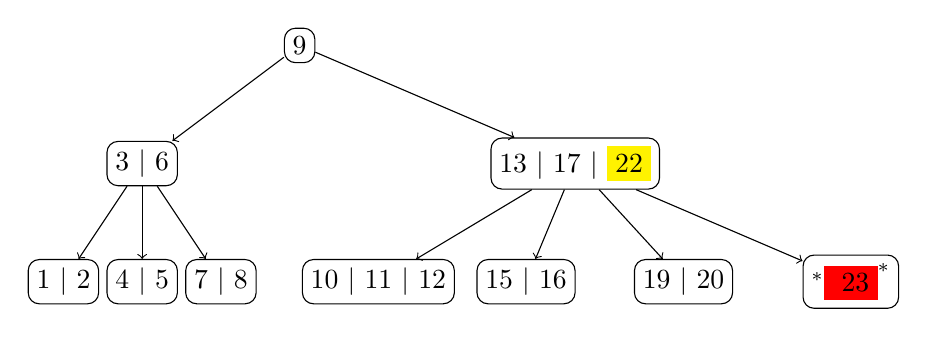
\begin{tikzpicture}
		\draw (1cm,2.0cm) node[inner sep = 3pt,draw,rounded corners] (r1){$9$}
		(-1.0cm, 0.5cm) node[inner sep = 3pt, draw,rounded corners] (lc1) {$3\ | \ 6$}
		(-2cm, -1.0cm) node[inner sep = 3pt, draw,rounded corners] (llc1) {$1\ | \ 2$}
		(-1cm, -1.0cm) node[inner sep = 3pt, draw,rounded corners] (llc2) {$4\ | \ 5$}
		(0cm, -1.0cm) node[inner sep = 3pt, draw,rounded corners] (llc3) {$7\ | \ 8$}
		(4.5cm, 0.5cm) node[inner sep = 3pt, draw,rounded corners] (rc1) {$13\ |\ 17 \ | \ \colorbox{yellow}{22}$}
		(2cm, -1.0cm) node[inner sep = 3pt, draw,rounded corners] (rrc1) {$10\ | \ 11\ | \ 12$}
		(3.875cm, -1.0cm) node[inner sep = 3pt, draw,rounded corners] (rrc2) {$15\ | \ 16$}
		(5.875cm, -1.0cm) node[inner sep = 3pt, draw,rounded corners] (rrc3) {$ 19\ | \ 20$}
		(8cm, -1.0cm) node[inner sep = 3pt, draw,rounded corners] (rrc4) {$^\ast\colorbox{red}{ 23}^\ast$};
		
		\draw[->] (r1) -- (lc1);
		\draw[->] (r1) -- (rc1);
		\draw[->] (lc1) -- (llc1);
		\draw[->] (lc1) -- (llc2);
		\draw[->] (lc1) -- (llc3);
		\draw[->] (rc1) -- (rrc1);
		\draw[->] (rc1) -- (rrc2);
		\draw[->] (rc1) -- (rrc3);
		\draw[->] (rc1) -- (rrc4);
	\end{tikzpicture}
\end{frame}

\begin{frame}{Observing that \texttt{leftSibling} has exactly $m=2$ keys, we cannot rotate, so we construct a \texttt{newNode} with exactly $2m=4$ keys by collapsing \texttt{currentNode} and \texttt{leftSibling}.}
	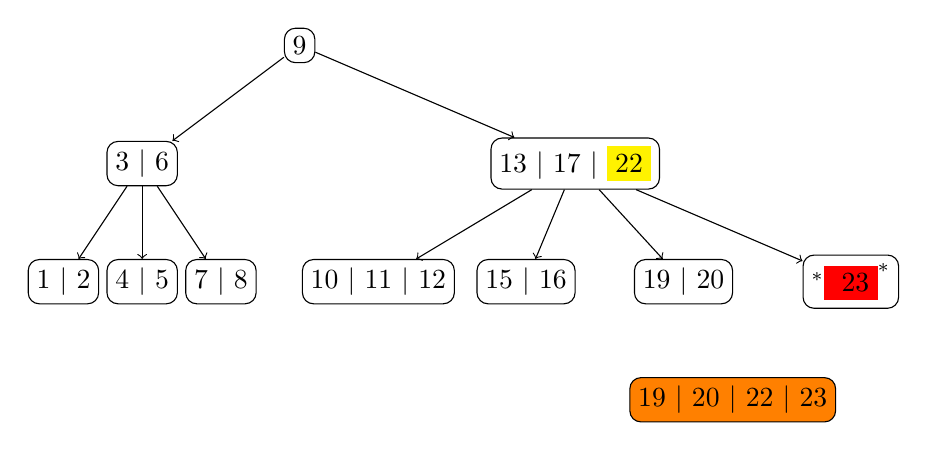
\begin{tikzpicture}
		\draw (1cm,2.0cm) node[inner sep = 3pt,draw,rounded corners] (r1){$9$}
		(-1.0cm, 0.5cm) node[inner sep = 3pt, draw,rounded corners] (lc1) {$3\ | \ 6$}
		(-2cm, -1.0cm) node[inner sep = 3pt, draw,rounded corners] (llc1) {$1\ | \ 2$}
		(-1cm, -1.0cm) node[inner sep = 3pt, draw,rounded corners] (llc2) {$4\ | \ 5$}
		(0cm, -1.0cm) node[inner sep = 3pt, draw,rounded corners] (llc3) {$7\ | \ 8$}
		(4.5cm, 0.5cm) node[inner sep = 3pt, draw,rounded corners] (rc1) {$13\ |\ 17 \ | \ \colorbox{yellow}{22}$}
		(2cm, -1.0cm) node[inner sep = 3pt, draw,rounded corners] (rrc1) {$10\ | \ 11\ | \ 12$}
		(3.875cm, -1.0cm) node[inner sep = 3pt, draw,rounded corners] (rrc2) {$15\ | \ 16$}
		(5.875cm, -1.0cm) node[inner sep = 3pt, draw,rounded corners] (rrc3) {$ 19\ | \ 20$}
		(8cm, -1.0cm) node[inner sep = 3pt, draw,rounded corners] (rrc4) {$^\ast\colorbox{red}{ 23}^\ast$}
		(6.5cm, -2.5cm) node[inner sep = 3pt, draw,rounded corners,fill = orange] (rrrc1) {$ 19\ | \ 20\ | \ 22\  | \ 23$};
		
		\draw[->] (r1) -- (lc1);
		\draw[->] (r1) -- (rc1);
		\draw[->] (lc1) -- (llc1);
		\draw[->] (lc1) -- (llc2);
		\draw[->] (lc1) -- (llc3);
		\draw[->] (rc1) -- (rrc1);
		\draw[->] (rc1) -- (rrc2);
		\draw[->] (rc1) -- (rrc3);
		\draw[->] (rc1) -- (rrc4);
	\end{tikzpicture}
\end{frame}
\begin{frame}{We then delete \texttt{currentNode}, delete \texttt{leftSibling} and delete the separater from \texttt{parent}. Then we link the gap in \texttt{parent} to \texttt{newNode}.}
	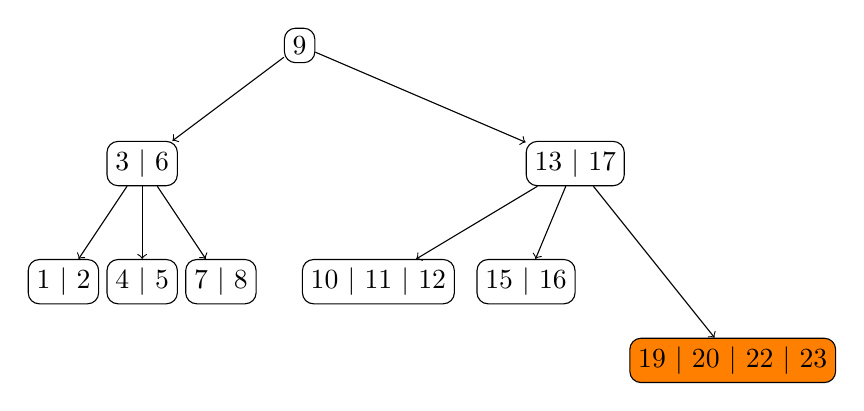
\begin{tikzpicture}
		\draw (1cm,2.0cm) node[inner sep = 3pt,draw,rounded corners] (r1){$9$}
		(-1.0cm, 0.5cm) node[inner sep = 3pt, draw,rounded corners] (lc1) {$3\ | \ 6$}
		(-2cm, -1.0cm) node[inner sep = 3pt, draw,rounded corners] (llc1) {$1\ | \ 2$}
		(-1cm, -1.0cm) node[inner sep = 3pt, draw,rounded corners] (llc2) {$4\ | \ 5$}
		(0cm, -1.0cm) node[inner sep = 3pt, draw,rounded corners] (llc3) {$7\ | \ 8$}
		(4.5cm, 0.5cm) node[inner sep = 3pt, draw,rounded corners] (rc1) {$13\ |\ 17$}
		(2cm, -1.0cm) node[inner sep = 3pt, draw,rounded corners] (rrc1) {$10\ | \ 11\ | \ 12$}
		(3.875cm, -1.0cm) node[inner sep = 3pt, draw,rounded corners] (rrc2) {$15\ | \ 16$}
		(6.5cm, -2cm) node[inner sep = 3pt, draw,rounded corners,fill = orange] (rrrc1) {$ 19\ | \ 20\ | \ 22\  | \ 23$};
		
		\draw[->] (r1) -- (lc1);
		\draw[->] (r1) -- (rc1);
		\draw[->] (lc1) -- (llc1);
		\draw[->] (lc1) -- (llc2);
		\draw[->] (lc1) -- (llc3);
		\draw[->] (rc1) -- (rrc1);
		\draw[->] (rc1) -- (rrc2);
		\draw[->] (rc1) -- (rrrc1);
	\end{tikzpicture}
\end{frame}
\begin{frame}{Lastly, we check for underflow at \texttt{parent}, but since $2\geq m =2$, there is no underflow, and we are done.}
	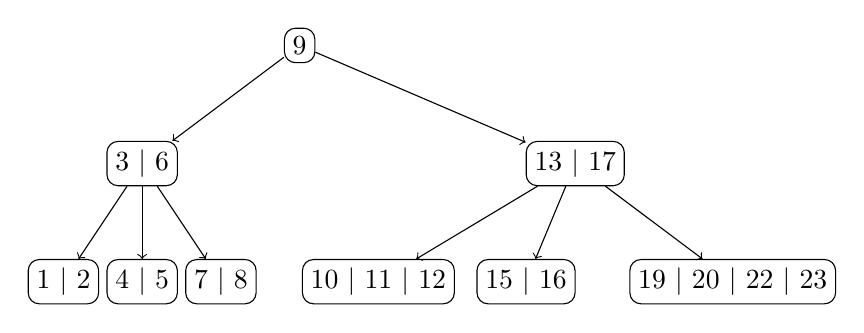
\begin{tikzpicture}
		\draw (1cm,2.0cm) node[inner sep = 3pt,draw,rounded corners] (r1){$9$}
		(-1.0cm, 0.5cm) node[inner sep = 3pt, draw,rounded corners] (lc1) {$3\ | \ 6$}
		(-2cm, -1.0cm) node[inner sep = 3pt, draw,rounded corners] (llc1) {$1\ | \ 2$}
		(-1cm, -1.0cm) node[inner sep = 3pt, draw,rounded corners] (llc2) {$4\ | \ 5$}
		(0cm, -1.0cm) node[inner sep = 3pt, draw,rounded corners] (llc3) {$7\ | \ 8$}
		(4.5cm, 0.5cm) node[inner sep = 3pt, draw,rounded corners] (rc1) {$13\ |\ 17$}
		(2cm, -1.0cm) node[inner sep = 3pt, draw,rounded corners] (rrc1) {$10\ | \ 11\ | \ 12$}
		(3.875cm, -1.0cm) node[inner sep = 3pt, draw,rounded corners] (rrc2) {$15\ | \ 16$}
		(6.5cm, -1cm) node[inner sep = 3pt, draw,rounded corners,] (rrc3) {$ 19\ | \ 20\ | \ 22\  | \ 23$};
		
		\draw[->] (r1) -- (lc1);
		\draw[->] (r1) -- (rc1);
		\draw[->] (lc1) -- (llc1);
		\draw[->] (lc1) -- (llc2);
		\draw[->] (lc1) -- (llc3);
		\draw[->] (rc1) -- (rrc1);
		\draw[->] (rc1) -- (rrc2);
		\draw[->] (rc1) -- (rrc3);
	\end{tikzpicture}
\end{frame}

\begin{frame}{Next we delete key 1, which we can do as it is a leaf node. This leaves underflow at \texttt{currentNode}.  We look to \texttt{rightSibling} and see that it doesn't have more than $m=2$ keys.}
	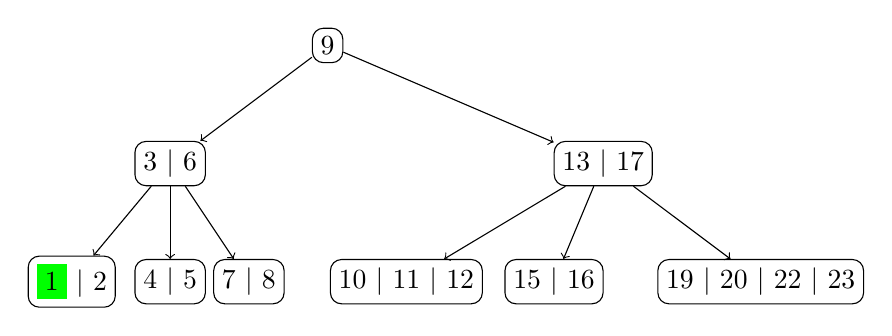
\begin{tikzpicture}
		\draw (1cm,2.0cm) node[inner sep = 3pt,draw,rounded corners] (r1){$9$}
		(-1.0cm, 0.5cm) node[inner sep = 3pt, draw,rounded corners] (lc1) {$3\ | \ 6$}
		(-2.25cm, -1.0cm) node[inner sep = 3pt, draw,rounded corners] (llc1) {$\colorbox{green}{1}\ | \ 2$}
		(-1cm, -1.0cm) node[inner sep = 3pt, draw,rounded corners] (llc2) {$4\ | \ 5$}
		(0cm, -1.0cm) node[inner sep = 3pt, draw,rounded corners] (llc3) {$7\ | \ 8$}
		(4.5cm, 0.5cm) node[inner sep = 3pt, draw,rounded corners] (rc1) {$13\ |\ 17$}
		(2cm, -1.0cm) node[inner sep = 3pt, draw,rounded corners] (rrc1) {$10\ | \ 11\ | \ 12$}
		(3.875cm, -1.0cm) node[inner sep = 3pt, draw,rounded corners] (rrc2) {$15\ | \ 16$}
		(6.5cm, -1cm) node[inner sep = 3pt, draw,rounded corners,] (rrc3) {$ 19\ | \ 20\ | \ 22\  | \ 23$};
		
		\draw[->] (r1) -- (lc1);
		\draw[->] (r1) -- (rc1);
		\draw[->] (lc1) -- (llc1);
		\draw[->] (lc1) -- (llc2);
		\draw[->] (lc1) -- (llc3);
		\draw[->] (rc1) -- (rrc1);
		\draw[->] (rc1) -- (rrc2);
		\draw[->] (rc1) -- (rrc3);
	\end{tikzpicture}
\end{frame}
\begin{frame}{Since a rotation is not possible, we collapse \texttt{currentNode} and \texttt{rightSibling}.}
	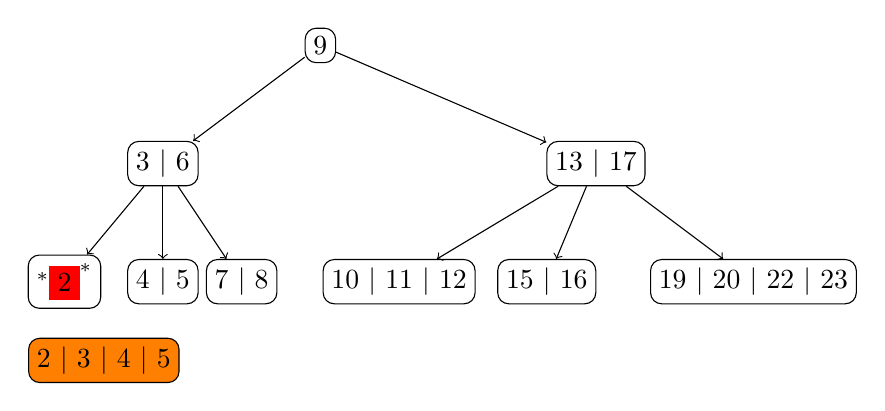
\begin{tikzpicture}
		\draw (1cm,2.0cm) node[inner sep = 3pt,draw,rounded corners] (r1){$9$}
		(-1.0cm, 0.5cm) node[inner sep = 3pt, draw,rounded corners] (lc1) {$3\ | \ 6$}
		(-2.25cm, -1.0cm) node[inner sep = 3pt, draw,rounded corners] (llc1) {$^\ast\colorbox{red}{2}^\ast$}
		(-1cm, -1.0cm) node[inner sep = 3pt, draw,rounded corners] (llc2) {$4\ | \ 5$}
		(0cm, -1.0cm) node[inner sep = 3pt, draw,rounded corners] (llc3) {$7\ | \ 8$}
		(-1.75cm, -2.0cm) node[inner sep = 3pt, draw,rounded corners, fill = orange] (lllc1) {$2\ | \ 3\ | \ 4\ | \ 5$}
		(4.5cm, 0.5cm) node[inner sep = 3pt, draw,rounded corners] (rc1) {$13\ |\ 17$}
		(2cm, -1.0cm) node[inner sep = 3pt, draw,rounded corners] (rrc1) {$10\ | \ 11\ | \ 12$}
		(3.875cm, -1.0cm) node[inner sep = 3pt, draw,rounded corners] (rrc2) {$15\ | \ 16$}
		(6.5cm, -1cm) node[inner sep = 3pt, draw,rounded corners] (rrc3) {$ 19\ | \ 20\ | \ 22\  | \ 23$};
		
		\draw[->] (r1) -- (lc1);
		\draw[->] (r1) -- (rc1);
		\draw[->] (lc1) -- (llc1);
		\draw[->] (lc1) -- (llc2);
		\draw[->] (lc1) -- (llc3);
		\draw[->] (rc1) -- (rrc1);
		\draw[->] (rc1) -- (rrc2);
		\draw[->] (rc1) -- (rrc3);
	\end{tikzpicture}
\end{frame}
\begin{frame}{When we are done linking the gap from \texttt{newNode} to \texttt{parent}, we then check overflow for \texttt{parent}, which it unfortunately is underflowing.}
	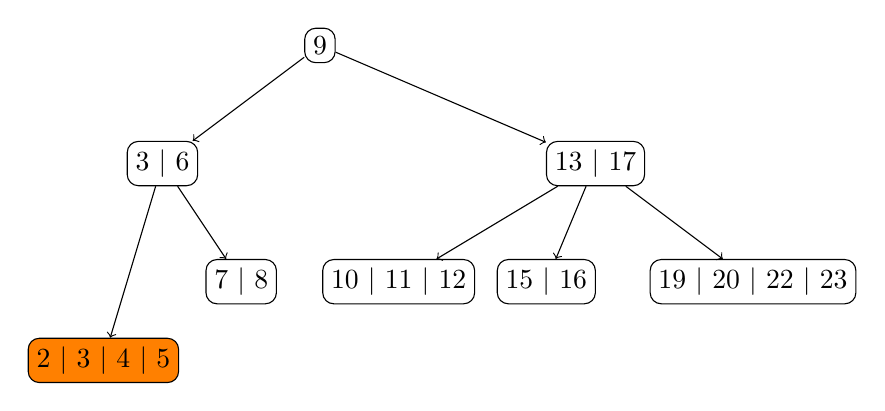
\begin{tikzpicture}
		\draw (1cm,2.0cm) node[inner sep = 3pt,draw,rounded corners] (r1){$9$}
		(-1.0cm, 0.5cm) node[inner sep = 3pt, draw,rounded corners] (lc1) {$3\ | \ 6$}
		(0cm, -1.0cm) node[inner sep = 3pt, draw,rounded corners] (llc3) {$7\ | \ 8$}
		(-1.75cm, -2.0cm) node[inner sep = 3pt, draw,rounded corners, fill = orange] (llc1) {$2\ | \ 3\ | \ 4\ | \ 5$}
		(4.5cm, 0.5cm) node[inner sep = 3pt, draw,rounded corners] (rc1) {$13\ |\ 17$}
		(2cm, -1.0cm) node[inner sep = 3pt, draw,rounded corners] (rrc1) {$10\ | \ 11\ | \ 12$}
		(3.875cm, -1.0cm) node[inner sep = 3pt, draw,rounded corners] (rrc2) {$15\ | \ 16$}
		(6.5cm, -1cm) node[inner sep = 3pt, draw,rounded corners] (rrc3) {$ 19\ | \ 20\ | \ 22\  | \ 23$};
		
		\draw[->] (r1) -- (lc1);
		\draw[->] (r1) -- (rc1);
		\draw[->] (lc1) -- (llc1);
		\draw[->] (lc1) -- (llc3);
		\draw[->] (rc1) -- (rrc1);
		\draw[->] (rc1) -- (rrc2);
		\draw[->] (rc1) -- (rrc3);
	\end{tikzpicture}
\end{frame}


\begin{frame}{Since we are underflowing at \texttt{parent}, and \texttt{rightSibling} cannot help, we must collapse \texttt{parent} and \texttt{rightSibling}, to finally arrive at the finished B-tree.}
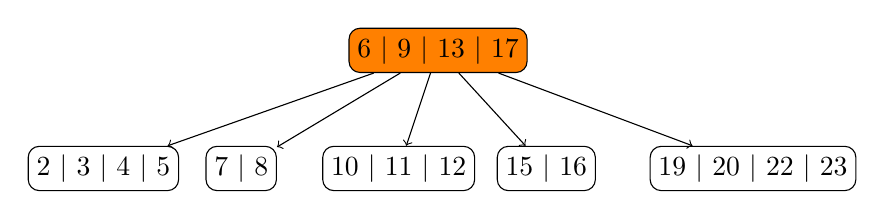
\begin{tikzpicture}
	\draw (0cm, -1.0cm) node[inner sep = 3pt, draw,rounded corners] (lc2) {$7\  | \ 8$}
	(-1.75cm, -1.0cm) node[inner sep = 3pt, draw,rounded corners] (lc1) {$2\ | \ 3\  | \ 4\  | \ 5$}
	(2.5cm, 0.5cm) node[inner sep = 3pt, draw,rounded corners,fill = orange] (r1) {$6\  | \ 9\  | \ 13\ | \ 17$}
	(2cm, -1.0cm) node[inner sep = 3pt, draw,rounded corners] (rc1) {$10\ | \ 11\ | \ 12$}
	(3.875cm, -1.0cm) node[inner sep = 3pt, draw,rounded corners] (rc2) {$15\ | \ 16$}
	(6.5cm, -1cm) node[inner sep = 3pt, draw,rounded corners] (rc3) {$ 19\ | \ 20\ | \ 22\  | \ 23$};
	
	\draw[->] (r1) -- (lc1);
	\draw[->] (r1) -- (lc2);
	\draw[->] (r1) -- (rc1);
	\draw[->] (r1) -- (rc2);
	\draw[->] (r1) -- (rc3);
\end{tikzpicture}
\end{frame}
\begin{frame}{Lastly, we perform a sanity check to see that every node has between 2 and $2m=4$ keys, and the \texttt{parent} has 4 nodes and 5 children, so we are done.}
	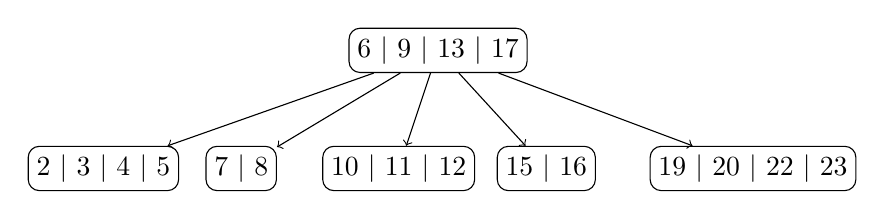
\begin{tikzpicture}
		\draw (0cm, -1.0cm) node[inner sep = 3pt, draw,rounded corners] (lc2) {$7\  | \ 8$}
		(-1.75cm, -1.0cm) node[inner sep = 3pt, draw,rounded corners] (lc1) {$2\ | \ 3\  | \ 4\  | \ 5$}
		(2.5cm, 0.5cm) node[inner sep = 3pt, draw,rounded corners] (r1) {$6\  | \ 9\  | \ 13\ | \ 17$}
		(2cm, -1.0cm) node[inner sep = 3pt, draw,rounded corners] (rc1) {$10\ | \ 11\ | \ 12$}
		(3.875cm, -1.0cm) node[inner sep = 3pt, draw,rounded corners] (rc2) {$15\ | \ 16$}
		(6.5cm, -1cm) node[inner sep = 3pt, draw,rounded corners] (rc3) {$ 19\ | \ 20\ | \ 22\  | \ 23$};
		
		\draw[->] (r1) -- (lc1);
		\draw[->] (r1) -- (lc2);
		\draw[->] (r1) -- (rc1);
		\draw[->] (r1) -- (rc2);
		\draw[->] (r1) -- (rc3);
	\end{tikzpicture}
\end{frame}
\end{document}
